%%%%%%%%%%%%%%%%%%%%%%%%%%%%%%%%%%%%%%%%%%%%%%%%%%%%%%%%%%%%%%%%%%%%%%%%%%%%%%%%%%
\begin{frame}[fragile]\frametitle{}
\begin{center}
{\Large PCA}
\end{center}
\end{frame}

%%%%%%%%%%%%%%%%%%%%%%%%%%%%%%%%%%%%%%%%%%%%%%%%%%%%%%%%%%
\begin{frame}[fragile]\frametitle{ Too much of anything is good for nothing!}
What happens when a data set has too many variables ? Here are few possible situations which you might come across:
\begin{itemize}
\item  You find that most of the variables are correlated.
\item  You lose patience and decide to run a model on whole data. This returns poor accuracy and you feel terrible.
\item  You become indecisive about what to do
\item  You start thinking of some strategic method to find few important variables
\end{itemize}
\end{frame}


%%%%%%%%%%%%%%%%%%%%%%%%%%%%%%%%%%%%%%%%%%%%%%%%%%%%%%%%%%%%%%%%%%%%%%%%%%%%%%%%%%
\begin{frame}[fragile]\frametitle{}
\begin{center}
{\Large High Dimensionality}
\end{center}
\end{frame}

%%%%%%%%%%%%%%%%%%%%%%%%%%%%%%%%%%%%%%%%%%%%%%%%%%%%%%%%%%
\begin{frame}[fragile]\frametitle{Curse	of Dimensionality}
\begin{itemize}
\item  Data-sets typically high dimensional	
 \item Images of 20x20 bitmaps have 400 dimensions. Mega pixel images has far too much.
 \item In text, all words are features, say, $10^6$.
\end{itemize}
\end{frame}


%%%%%%%%%%%%%%%%%%%%%%%%%%%%%%%%%%%%%%%%%%%%%%%%%%%%%%%%%%
\begin{frame}[fragile]\frametitle{Curse	of Dimensionality}
\begin{itemize}
 \item Machine Learning methods are statistical, and data sparse.
 \item As the Dimensionality grows, fewer observations per region, ie density.
 \item Actual/True content is in the very small subset of this high dimensional space.
 \item More dense the space, better for the algorithm.
\end{itemize}
\end{frame}



%%%%%%%%%%%%%%%%%%%%%%%%%%%%%%%%%%%%%%%%%%%%%%%%%%%%%%%%%%
\begin{frame}[fragile]\frametitle{ Dimensionality Reduction Algorithms}
\begin{itemize}
\item  How'd  you  identify  highly  significant variable(s) out 1000 or 2000?
\item Feature selection: Select only relevant features (based on domain, correlation, etc)
\item Feature Extraction: Compose new features based on combination of all existing ones.
\end{itemize}
\end{frame}


%%%%%%%%%%%%%%%%%%%%%%%%%%%%%%%%%%%%%%%%%%%%%%%%%%%%%%%%%%
\begin{frame}[fragile]\frametitle{ Dimensionality Reduction Algorithms}
\begin{itemize}
\item Principal Components Analysis (PCA) is a Feature Extraction method.
\item Projects data from high-dimensional space into a lower-dimensional space
% \item Not necessarily interested in ``losing information''; rather eliminate some of the sparsity
\end{itemize}
\end{frame}


% %%%%%%%%%%%%%%%%%%%%%%%%%%%%%%%%%%%%%%%%%%%%%%%%%%%%%%%%%%
% \begin{frame}[fragile]\frametitle{Feature Selection Methods}
% \begin{itemize}
% \item Manually via Data Analyst. Intuition about problem domain
% \item Systematic Approach: Try all possible combinations of feature subsets?. See which combination results in best model
% \item For n features, there are 2n possible combinations of subsets. Infeasible to try each of them
% \end{itemize}
% \end{frame}

% %%%%%%%%%%%%%%%%%%%%%%%%%%%%%%%%%%%%%%%%%%%%%%%%%%%%%%%%%%
% \begin{frame}[fragile]\frametitle{Feature Selection Methods}
% Feature Construction
% \begin{itemize}
% \item Example: combining two separate features (\# of full baths, \# of half baths) into one feature (``total baths'')
% \item Example: combining features (mass) and (volume) into one feature (density), where density = mass / volume
% \end{itemize}
% \end{frame}

% %%%%%%%%%%%%%%%%%%%%%%%%%%%%%%%%%%%%%%%%%%%%%%%%%%%%%%%%%%
% \begin{frame}[fragile]\frametitle{Feature Selection Methods}
% Feature Subset Selection
% \begin{itemize}
% \item Reducing number of features by only using a subset of features
% \item Losing information if we only consider a subset of features?
% \item By eliminating unnecessary features, we hope for a better model.
% \end{itemize}

% \end{frame}
% %%%%%%%%%%%%%%%%%%%%%%%%%%%%%%%%%%%%%%%%%%%%%%%%%%%%%%%%%%
% \begin{frame}[fragile]\frametitle{Three Systematic Approaches}
% \begin{itemize}
% \item Embedded Approaches
	% \begin{itemize}
	% \item Algorithm specific
	% \item Occurs naturally as part of the data mining algorithm. Example: present in decision tree induction
	% \end{itemize}
% \item Filter Approaches
	% \begin{itemize}
	% \item Features are selected before the data mining algorithm is run
	% \item Example: (trying to eliminate redundant features) Look at pairwise correlation between variables
	% \end{itemize}
% \item Wrapper Approaches
	% \begin{itemize}
	% \item Data mining algorithm is a “black box” for finding best subset of features
	% \item Final model uses the specific subset that evaluates the best
	% \end{itemize}
% \end{itemize}
% \end{frame}

% %%%%%%%%%%%%%%%%%%%%%%%%%%%%%%%%%%%%%%%%%%%%%%%%%%%%%%%%%%
% \begin{frame}[fragile]\frametitle{Top-Down Wrapper}
% \begin{itemize}
% \item Assuming n number of features
% \item Start with no attributes
% \item Train classifier n times, each time with a different feature
% \begin{itemize}
% \item Each classifier only has a single predictor
% \item See which of the n classifiers performs the best
% \end{itemize}
% \item Add to the best classifier. Recursively use remaining attributes to find which attribute that improves performance the most. Keep including best attribute 
% \item Stopping criterion:  Stop if no improvement to classifier performance, or increase in classifier performance is less than some threshold
% \end{itemize}
% \end{frame}


% %%%%%%%%%%%%%%%%%%%%%%%%%%%%%%%%%%%%%%%%%%%%%%%%%%%%%%%%%%
% \begin{frame}[fragile]\frametitle{Bottom-Up Wrapper}
% \begin{itemize}
% \item Assuming n number of features
% \item Start with all n attributes in model
% \item Create n models, each with a different predictor omitted.
% \begin{itemize}
% \item Each classifier has n-1 predictors
% \item See which of the n classifiers affects performance the least
% \item Throw that attribute out
% \end{itemize}
% \item Recursively find the attribute that affects performance the least
% \item Stopping criterion:  Stop if classifier performance begins to degrade
% \end{itemize}
% \end{frame}


% %%%%%%%%%%%%%%%%%%%%%%%%%%%%%%%%%%%%%%%%%%%%%%%%%%%
% \begin{frame}[fragile] \frametitle{} 

% As we have started to see, the curse of dimensionality stops
% us from being able to fit arbitrarily complex models in high
% dimensional spaces.

% \textbf{Additive models} try to avoid this by fixing the structure
% of the learned models to limit interactions between the input variables.

% \textbf{Tree-based models} attempt to use the data itself to greedily
% learn which interactions are actually important.

% \end{frame}

% %%%%%%%%%%%%%%%%%%%%%%%%%%%%%%%%%%%%%%%%%%%%%%%%%%%
% \begin{frame}[fragile] \frametitle{} 

% Today we are going to look at another technique called
% \textbf{principal components} (PCs), or principal component
% analysis (PCA), a specific example of dimensionality
% reduction.

% Like trees, these use the data to find lower dimensional structures
% hidden in higher dimensional space. They differ from trees, however,
% because principal components use \textbf{only the predictor variables} (not
% the responses) and attempt to capture \textbf{global and linear structure},
% rather than local ones.

% \end{frame}


%%%%%%%%%%%%%%%%%%%%%%%%%%%%%%%%%%%%%%%%%%%%%%%%%%%%%%%%%%%%%%%%%%%%%%%%%%%%%%%%%%
\begin{frame}[fragile]\frametitle{}
\begin{center}
{\Large Dimensionality Reduction Example}
\end{center}
\end{frame}

%%%%%%%%%%%%%%%%%%%%%%%%%%%%%%%%%%%%%%%%%%%%%%%%%%%
\begin{frame}[fragile] \frametitle{Body Measurements}

Say that we have a data-set of the following measurements from
a large set of human volunteers with the following variables:
\begin{itemize}
\item height
\item weight
\item waist size
\item shoe size
\item length of right arm
\item length of left arm

\end{itemize}

\end{frame}

%%%%%%%%%%%%%%%%%%%%%%%%%%%%%%%%%%%%%%%%%%%%%%%%%%%
\begin{frame}[fragile] \frametitle{Body Measurements}
\begin{itemize}
\item length of torso
% \item pant inseam length
\item hat size
\item left hand ring size
\item right hand ring size
\end{itemize}
Technically we have $10$ variables, though most of the variation
in the data-set can be summarized by at most 2-3 variables.

What can you do? Domain knowledge?
\end{frame}

%%%%%%%%%%%%%%%%%%%%%%%%%%%%%%%%%%%%%%%%%%%%%%%%%%%
\begin{frame}[fragile] \frametitle{Reduction in Dimensions} 
In decreasing order of variation, consider the following measurements
that can be derived from these $10$ variables
\begin{itemize}
\item height: captures a large amount of the variation in the total
dataset. 
\item body mass index: should be
relatively uncorrelated with overall height, captures much of the
next largest variation in the data. 
\item ratio of torso length to total height: attempts
to capture the remaining variation based on how height is distributed
over a given individuals frame.
\end{itemize}
\end{frame}

%%%%%%%%%%%%%%%%%%%%%%%%%%%%%%%%%%%%%%%%%%%%%%%%%%%%%%%%%%%%%%%%%%%%%%%%%%%%%%%%%%
\begin{frame}[fragile]\frametitle{}
\begin{center}
{\Large PCA Algorithm}
\end{center}
\end{frame}

%%%%%%%%%%%%%%%%%%%%%%%%%%%%%%%%%%%%%%%%%%%%%%%%%%%
\begin{frame}[fragile] \frametitle{PCA} 
\begin{itemize}
\item One of the oldest (1901!) 
\item To understand ``important'' dimensions
\end{itemize}
\end{frame}

%%%%%%%%%%%%%%%%%%%%%%%%%%%%%%%%%%%%%%%%%%%%%%%%%%%
\begin{frame}[fragile] \frametitle{PCA} 
\begin{itemize}
\item PCA looks at the data and tries to find a direction-line along which data is spread the most.
\item Once done, you look for another (perpendicular) dimension which has second most variation.
\item These are called as Principal components.
\end{itemize}
\end{frame}
%
%%%%%%%%%%%%%%%%%%%%%%%%%%%%%%%%%%%%%%%%%%%%%%%%%%%%
%\begin{frame}[fragile] \frametitle{PCA} 
%\begin{itemize}
%\item Each principal component, however, must be a linear function of the
%input variables (so BMI would not be allowed). 
%\item They all the data points are re-coded in terms of new basis vectors. A new coordinate system.
%\end{itemize}
%\end{frame}

%%%%%%%%%%%%%%%%%%%%%%%%%%%%%%%%%%%%%%%%%%%%%%%%%%%
\begin{frame}[fragile] \frametitle{PCA in a nutshell} 
\begin{center}
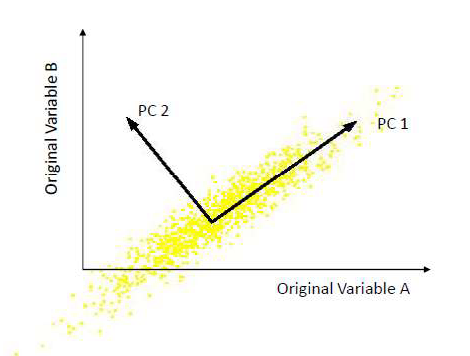
\includegraphics[width=0.6\linewidth,keepaspectratio]{pca6}
\end{center}
\begin{itemize}
\item Orthogonal directions of greatest variance in data
\item Projections along PC1 discriminate the data most along any one axis
\end{itemize}
\end{frame}

%%%%%%%%%%%%%%%%%%%%%%%%%%%%%%%%%%%%%%%%%%%%%%%%%%%
\begin{frame}[fragile] \frametitle{PCA} 
\begin{itemize}
\item  First principal component is the direction of greatest
variability (co-variance) in the data
\item Second is the next orthogonal (uncorrelated) direction of greatest variability. So first remove all the variability along the first
component, and then find the next direction of greatest variability 
\item  And so on
\end{itemize}
\end{frame}

%%%%%%%%%%%%%%%%%%%%%%%%%%%%%%%%%%%%%%%%%%%%%%%%%%%
\begin{frame}[fragile] \frametitle{PCA} 
 Principle
\begin{itemize}
\item   Linear projection method to reduce the number of parameters
\item   Transfer a set of correlated variables into a new set of uncorrelated variables
\item   Map the data into a space of lower Dimensionality
\item   Form of unsupervised learning
\end{itemize}
\end{frame}

%%%%%%%%%%%%%%%%%%%%%%%%%%%%%%%%%%%%%%%%%%%%%%%%%%%%
%\begin{frame}[fragile] \frametitle{PCA} 
% Properties
%\begin{itemize}
%\item   It can be viewed as a rotation of the existing axes to new positions in the 
%space defined by original variables
%\item   New axes are orthogonal and represent the directions with maximum 
%variability
%\end{itemize}
%\end{frame}
%%%%%%%%%%%%%%%%%%%%%%%%%%%%%%%%%%%%%%%%%%%%%%%%%%%
\begin{frame}[fragile] \frametitle{Why greatest variability?	} 
\adjustbox{valign=t}{
\begin{minipage}{0.5\linewidth}
\begin{itemize}
\item Example: reduce 2-dimensional data to 1
\item Data points in 2D $x_1,x_2$ space are represented by projection points on $z$ axis, so, only 1-D distances.
\item See how two red points on different z axes are ad different distances.
\item The one with max variance preserves original intent-structure.
%\item Variance = $ 1/n \sum (\sum projections - mean)^2$
\end{itemize}

\end{minipage}
}
\hfill
\adjustbox{valign=t}{
\begin{minipage}{0.4\linewidth}
\begin{center}
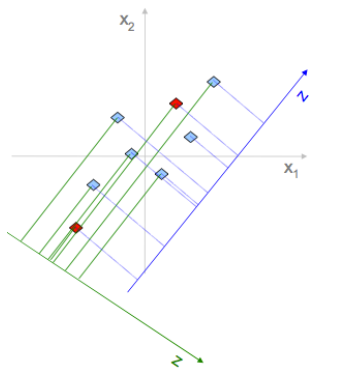
\includegraphics[width=\linewidth,keepaspectratio]{pca4}
\end{center}
%Remember Eigen values and vectors $| A - \lambda I | = 0$
\end{minipage}
}
\end{frame}

%%%%%%%%%%%%%%%%%%%%%%%%%%%%%%%%%%%%%%%%%%%%%%%%%%%%
%\begin{frame}[fragile] \frametitle{PCA} 
%\begin{itemize}
%\item    Finding $u$ such that $E(u.x)^2)$ is max for all $x$
%\item $E((u.x)^2) = E((u.x)(u.x)^T) = E(u.x.x^T.u^T)$
%\item Matrix $S = x.x^T$ contains the co-variances among pairs of x features, in the original coordinates system
%\item So we are looking to maximize $u.S.u^T$
%\end{itemize}
%\end{frame}

%%%%%%%%%%%%%%%%%%%%%%%%%%%%%%%%%%%%%%%%%%%%%%%%%%%%%%%%%%%%%%%%%%%%%%%%%%%%%%%%%%
\begin{frame}[fragile]\frametitle{}
\begin{center}
{\Large PCA in Steps}
\end{center}
\end{frame}

%%%%%%%%%%%%%%%%%%%%%%%%%%%%%%%%%%%%%%%%%%%%%%%%%%%
\begin{frame}[fragile] \frametitle{PCA in Steps} 
\begin{itemize}
\item Center the data by subtracting mean.
\item Subtracting the mean makes variance and covariance 
calculation easier by simplifying their equations. 
\item The 
variance and co-variance values are not affected by 
the mean value.
\item Compute Co-variance matrix.
\end{itemize}
\end{frame}


%%%%%%%%%%%%%%%%%%%%%%%%%%%%%%%%%%%%%%%%%%%%%%%%%%%
\begin{frame}[fragile] \frametitle{PCA in Steps} 
\begin{center}
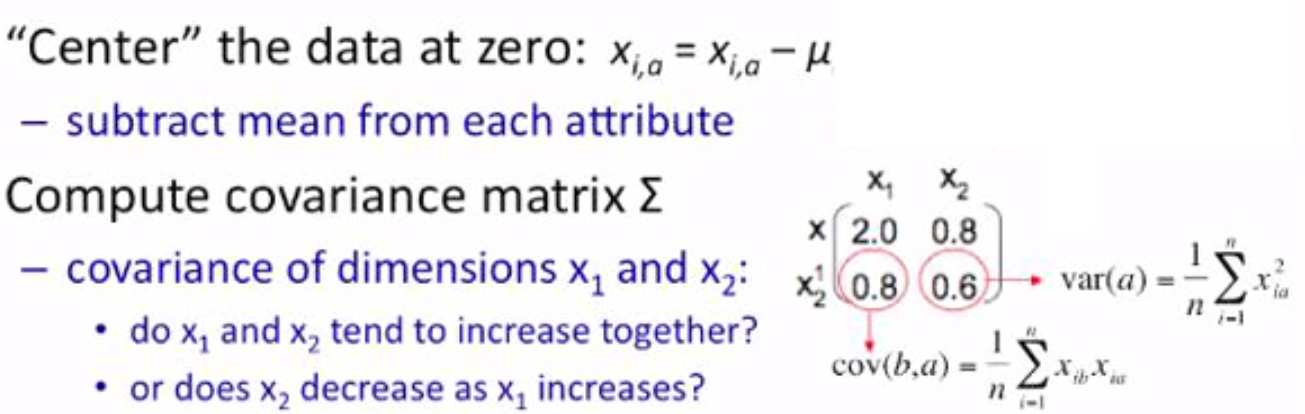
\includegraphics[width=\linewidth,keepaspectratio]{pca19}
\end{center}
\tiny{(Reference: Principal Component Analysis - Victor Lavrenko)}
\end{frame}

%%%%%%%%%%%%%%%%%%%%%%%%%%%%%%%%%%%%%%%%%%%%%%%%%%%
\begin{frame}[fragile] \frametitle{PCA in Steps} 
First way
\begin{itemize}
\item Initialize seed vector
\item Successive multiplication with Co-variance matrix
\item Transforms the vector 
\item Finally, the Principal Components.
\end{itemize}
\begin{center}
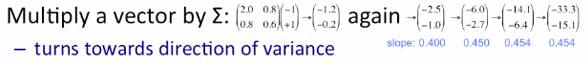
\includegraphics[width=\linewidth,keepaspectratio]{pca20}
\end{center}
\end{frame}


%%%%%%%%%%%%%%%%%%%%%%%%%%%%%%%%%%%%%%%%%%%%%%%%%%%
\begin{frame}[fragile] \frametitle{PCA in Steps} 
Another way
\begin{itemize}
\item Calculate the eigen vectors and eigenvalues of 
the co-variance matrix (Manually, Python, Matlab, etc)
\item Since the non-diagonal elements in this co-variance 
matrix are positive, we should expect that both the x 
and y variable increase together.
\end{itemize}
\begin{center}
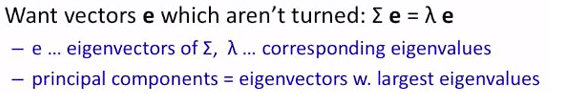
\includegraphics[width=\linewidth,keepaspectratio]{pca21}
\end{center}
\end{frame}


%%%%%%%%%%%%%%%%%%%%%%%%%%%%%%%%%%%%%%%%%%%%%%%%%%%
\begin{frame}[fragile] \frametitle{PCA in Steps} 
\begin{itemize}
\item Retain top Principal components 
\item Project original X data on them
\end{itemize}
\end{frame}

% %%%%%%%%%%%%%%%%%%%%%%%%%%%%%%%%%%%%%%%%%%%%%%%%%%%%%%%%%%%%%%%%%%%%%%%%%%%%%%%%%%
% \begin{frame}[fragile]\frametitle{}
% \begin{center}
% {\Large PCA Graphically}
% \end{center}
% \end{frame}

% %%%%%%%%%%%%%%%%%%%%%%%%%%%%%%%%%%%%%%%%%%%%%%%%%%%
% \begin{frame}[fragile] \frametitle{Geometric view of PCA}
% Goal:  Find variation in data with as less components as possible
% \begin{center}
% 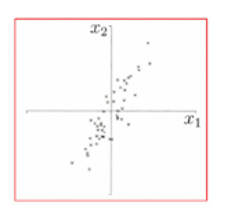
\includegraphics[width=0.6\linewidth,keepaspectratio]{pca10}
% \end{center}
% \end{frame}

% %%%%%%%%%%%%%%%%%%%%%%%%%%%%%%%%%%%%%%%%%%%%%%%%%%%
% \begin{frame}[fragile] \frametitle{Geometric view of PCA}
% Try directions, pick the one giving max variance
% \begin{center}
% 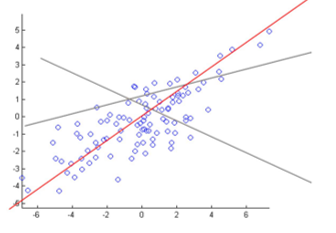
\includegraphics[width=0.6\linewidth,keepaspectratio]{pca11}
% \end{center}
% \end{frame}

% %%%%%%%%%%%%%%%%%%%%%%%%%%%%%%%%%%%%%%%%%%%%%%%%%%%
% \begin{frame}[fragile] \frametitle{Geometric view of PCA}
% Again try directions, pick the next one giving max variance
% \begin{center}
% 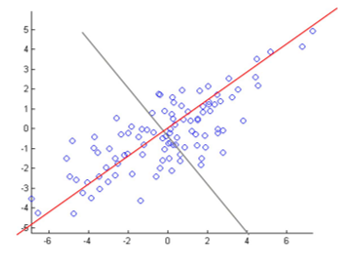
\includegraphics[width=0.6\linewidth,keepaspectratio]{pca12}
% \end{center}
% \end{frame}

% %%%%%%%%%%%%%%%%%%%%%%%%%%%%%%%%%%%%%%%%%%%%%%%%%%%
% \begin{frame}[fragile] \frametitle{Geometric view of PCA}
% \begin{itemize}
% \item 1st Direction: maximum variance
% \item 2nd Direction: Perpendicular to first, with next max variance
% \end{itemize}
% \begin{center}
% 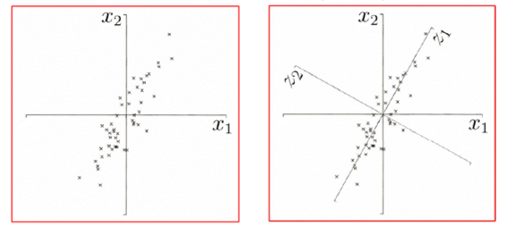
\includegraphics[width=0.8\linewidth,keepaspectratio]{pca13}
% \end{center}
% \end{frame}

%%%%%%%%%%%%%%%%%%%%%%%%%%%%%%%%%%%%%%%%%%%%%%%%%%%%%%%%%%%%%%%%%%%%%%%%%%%%%%%%%%
\begin{frame}[fragile]\frametitle{}
\begin{center}
{\Large PCA Example Working}
\end{center}
\end{frame}


%%%%%%%%%%%%%%%%%%%%%%%%%%%%%%%%%%%%%%%%%%%%%%%%%%%
\begin{frame}[fragile] \frametitle{PCA Example in Steps} 
Subtract the mean
\begin{itemize}
\item From each of the data dimensions. 
\item All the $x$ values have their $\bar{x}$ subtracted and $y$ values have $\bar{y}$ subtracted 
from them. 
\item This produces a data set whose mean is zero.
\item Subtracting the mean makes variance and covariance 
calculation easier by simplifying their equations. 
\item The 
variance and co-variance values are not affected by 
the mean value.
\end{itemize}
\end{frame}


%%%%%%%%%%%%%%%%%%%%%%%%%%%%%%%%%%%%%%%%%%%%%%%%%%%
\begin{frame}[fragile] \frametitle{PCA Example in Steps} 
\begin{center}
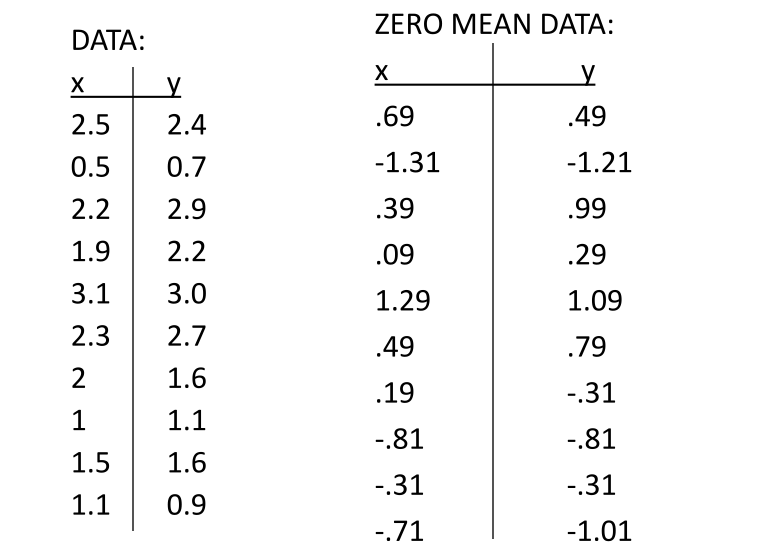
\includegraphics[width=0.8\linewidth,keepaspectratio]{pca8}
\end{center}
\end{frame}

%%%%%%%%%%%%%%%%%%%%%%%%%%%%%%%%%%%%%%%%%%%%%%%%%%%
\begin{frame}[fragile] \frametitle{PCA Example in Steps} 
Original Data
\begin{center}
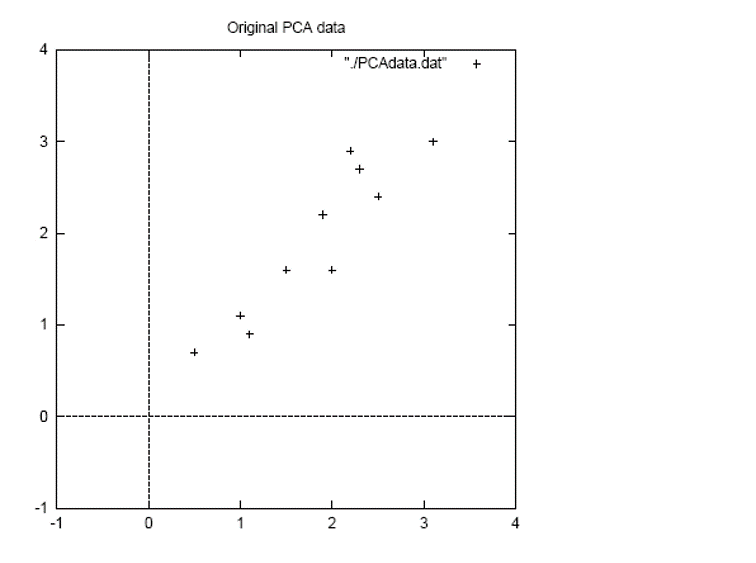
\includegraphics[width=0.8\linewidth,keepaspectratio]{pca14}
\end{center}
\end{frame}


%%%%%%%%%%%%%%%%%%%%%%%%%%%%%%%%%%%%%%%%%%%%%%%%%%%
\begin{frame}[fragile] \frametitle{PCA Example in Steps} 
\begin{itemize}
\item Calculate the co-variance matrix (Manually, Python, Matlab, etc)
\begin{center}
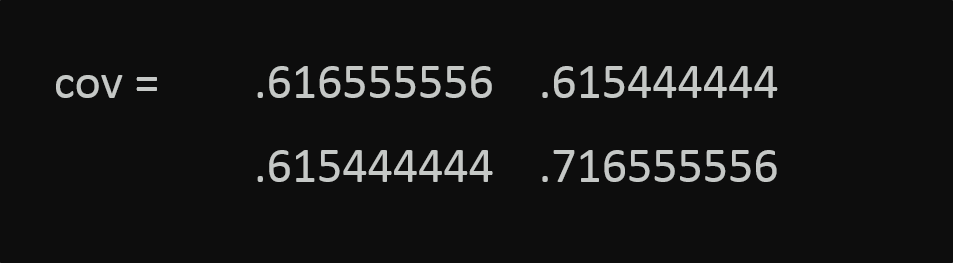
\includegraphics[width=0.8\linewidth,keepaspectratio]{pca9}
\end{center}
\item Since the non-diagonal elements in this co-variance 
matrix are positive, we should expect that both the x 
and y variable increase together.
\end{itemize}
\end{frame}

%%%%%%%%%%%%%%%%%%%%%%%%%%%%%%%%%%%%%%%%%%%%%%%%%%%
\begin{frame}[fragile] \frametitle{PCA Example in Steps} 
\begin{itemize}
\item Calculate the eigen-vectors and eigenvalues of the co-variance  (Manually, Python, Matlab, etc)
\begin{center}
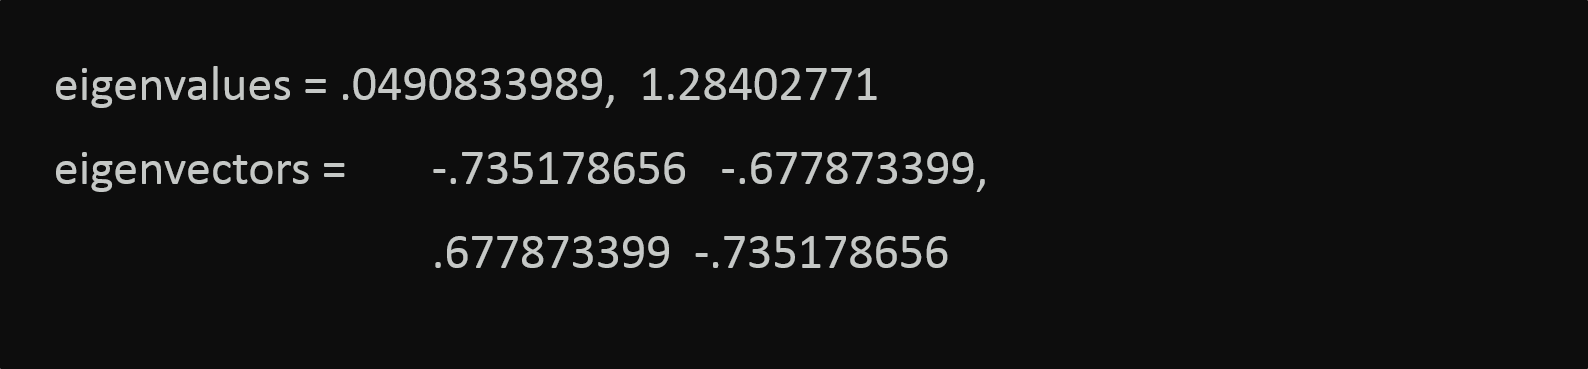
\includegraphics[width=0.8\linewidth,keepaspectratio]{pca15}
\end{center}
\item Note they are perpendicular to each other
\end{itemize}
\end{frame}

%%%%%%%%%%%%%%%%%%%%%%%%%%%%%%%%%%%%%%%%%%%%%%%%%%%
\begin{frame}[fragile] \frametitle{PCA Example in Steps} 
\begin{itemize}
\item Highest eigenvalue is the principle component.
\item Here, it is pointed down the middle of the data. 
\item Order eigen vectors by eigenvalue, highest to lowest. 
\item The order of significance. 
\item Keep important ones. 
\item Small eigenvalues ignorable
\end{itemize}
\end{frame}

%%%%%%%%%%%%%%%%%%%%%%%%%%%%%%%%%%%%%%%%%%%%%%%%%%%
\begin{frame}[fragile] \frametitle{PCA Example in Steps} 
$NewData = RowFeatureVector_{nf \times nf} \times RowZeroMeanData_{nRows \times nf transposed}$
\begin{itemize}
\item RowFeatureVector: Matrix with eigen-vectors as rows, first on top
\item RowZeroMeanData is the mean-adjusted data transposed
\end{itemize}
\end{frame}

%%%%%%%%%%%%%%%%%%%%%%%%%%%%%%%%%%%%%%%%%%%%%%%%%%%
\begin{frame}[fragile] \frametitle{PCA Example in Steps} 
\begin{center}
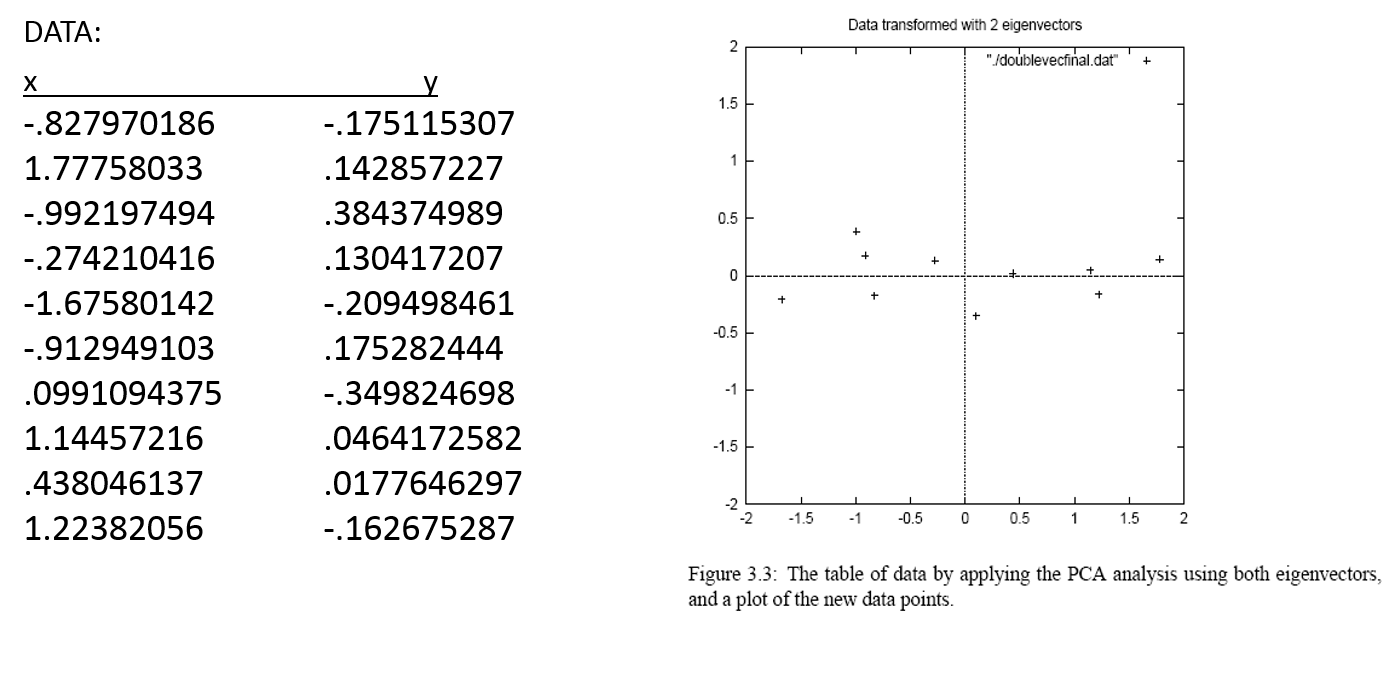
\includegraphics[width=\linewidth,keepaspectratio]{pca16}
\end{center}
\end{frame}



%%%%%%%%%%%%%%%%%%%%%%%%%%%%%%%%%%%%%%%%%%%%%%%%%%%
\begin{frame}[fragile] \frametitle{PCA in a nutshell} 
\begin{center}
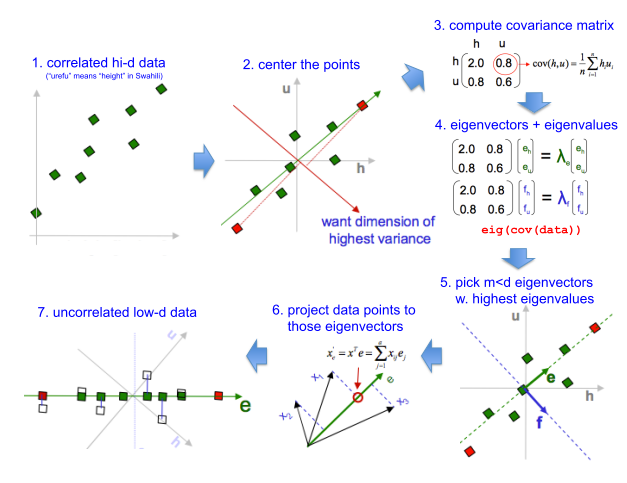
\includegraphics[width=0.8\linewidth,keepaspectratio]{pca5}
\end{center}
\end{frame}


%%%%%%%%%%%%%%%%%%%%%%%%%%%%%%%%%%%%%%%%%%%%%%%%%%%%
%\begin{frame}[fragile] \frametitle{PCA} 
%The image below shows the transformation of a high dimensional data (3 dimension) to low dimensional data (2 dimension) using PCA. Not to forget, each resultant dimension is a linear combination of p features
%\begin{center}
%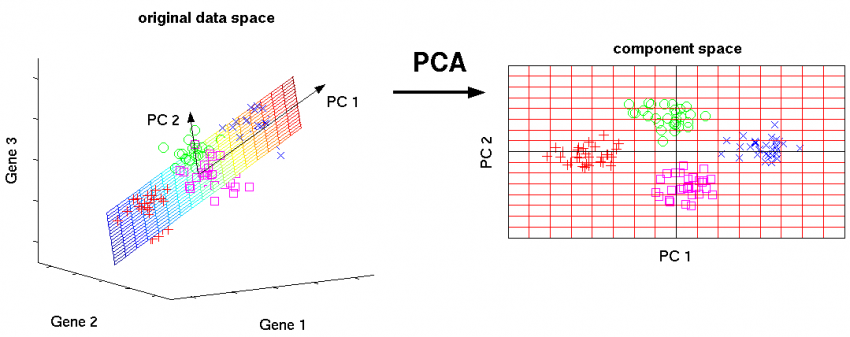
\includegraphics[width=\linewidth,keepaspectratio]{pca2}
%\end{center}
%\end{frame}


%%%%%%%%%%%%%%%%%%%%%%%%%%%%%%%%%%%%%%%%%%%%%%%%%%%
\begin{frame}[fragile] \frametitle{PCA} 

\begin{itemize}
\item A principal component is a normalized linear combination of the original predictors in a data set.
\item The first principal component can be written as:
$Z^1 = w^{11}X^1 + w^{21}X^2 + \ldots +  w^{p1}X^p$
\item It captures the maximum variance in the data set. 
\item It determines the direction of highest variability in the data. 
\item Larger the variability captured in first component, larger the information captured by component. 
\item No other component can have variability higher than first principal component.
\end{itemize}
\end{frame}

%%%%%%%%%%%%%%%%%%%%%%%%%%%%%%%%%%%%%%%%%%%%%%%%%%%
\begin{frame}[fragile] \frametitle{PCA} 

\begin{itemize}
\item The first principal component results in a line which is closest to the data i.e. it minimizes the sum of squared distance between a data point and the line.
\item Similarly, we can compute the second principal component also.
$Z^2 = w^{12}X^1 + w^{22}X^2 + \ldots +  w^{p2}X^p$
\item If the two components are uncorrelated, their directions should be orthogonal
\begin{center}
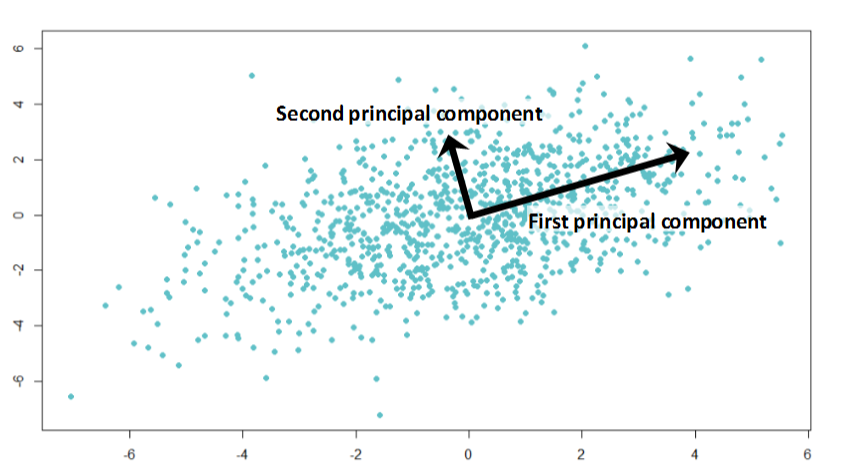
\includegraphics[width=0.7\linewidth,keepaspectratio]{pca3}
\end{center}
\item All succeeding principal component capture the remaining variation without being correlated with the previous component. 
\end{itemize}

\end{frame}


%%%%%%%%%%%%%%%%%%%%%%%%%%%%%%%%%%%%%%%%%%%%%%%%%%%
\begin{frame}[fragile] \frametitle{PCA} 
Can ignore the components of lesser significance.
\begin{center}
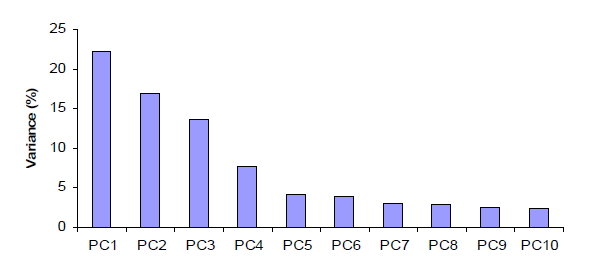
\includegraphics[width=\linewidth,keepaspectratio]{pca7}
\end{center}
You do lose some information, but if the eigenvalues are small, you don't lose 
much.
\end{frame}

%%%%%%%%%%%%%%%%%%%%%%%%%%%%%%%%%%%%%%%%%%%%%%%%%%%%
%\begin{frame}[fragile] \frametitle{Principal components} 
%
%Formally, the principal components of the matrix $X$ are a linear
%re-parametrization $T=wX$ of the matrix $X$. The first column of
%$T$ is the first principal component, the second column is the second
%principal component, and so on.
%
%\end{frame}

%%%%%%%%%%%%%%%%%%%%%%%%%%%%%%%%%%%%%%%%%%%%%%%%%%%%
%\begin{frame}[fragile] \frametitle{Principal components} 
%
%Specifically, the matrix $w$ is defined uniquely by the following
%conditions:
%\begin{itemize}
%\item Each column of $T$ must be uncorrelated with the others;
%specifically, $w$ is an orthogonal matrix called the \textit{loadings}
%\item The first column of $T$ has the largest variance of all
%linear combinations of the columns of X, the second column has the
%highest variance conditioned on being uncorrelated with the
%first, and so forth.
%\end{itemize}
%
%\end{frame}
%
%
%%%%%%%%%%%%%%%%%%%%%%%%%%%%%%%%%%%%%%%%%%%%%%%%%%%%
%\begin{frame}[fragile] \frametitle{Mathematically} 
%
%\begin{itemize}
%\item 
%It can be shown that the matrix $w$ is equal to the eigenvectors
%of the matrix $X^tX$. 
%\item From this relationship, there are many
%results from numerical linear algebra that can be used to develop
%theoretical results about principal components.
%\end{itemize}
%\end{frame}

%%%%%%%%%%%%%%%%%%%%%%%%%%%%%%%%%%%%%%%%%%%%%%%%%%%
\begin{frame}[fragile]
\frametitle{Principal Component Analysis}
Advantages
\begin{itemize}
	\item Useful Pre-processing step
	\item Reduces computational complexity
	\item Noise reduction
\end{itemize}
\end{frame}

%%%%%%%%%%%%%%%%%%%%%%%%%%%%%%%%%%%%%%%%%%%%%%%%%%%
\begin{frame}[fragile]
\frametitle{Principal Component Analysis}
Limitations
\begin{itemize}
	\item Linear manifold only
	\item 
Co-variance Matrix huge, finding eigen-vectors is slow
	\item 
SVD comes to rescue

\end{itemize}
\end{frame}



%%%%%%%%%%%%%%%%%%%%%%%%%%%%%%%%%%%%%%%%%%%%%%%%%%%%
%\begin{frame}[fragile] \frametitle{A look ahead} 
%
%The main shortcoming of principal components are that they only
%capture global linear structures in the data. This tends to be
%a larger problem for prediction than it is for visualization.
%
%Figuring out how to get non-linear extensions of principal
%components is a wide open problem in statistic and machine learning.
%Some avenues of research include:
%\begin{itemize}
%\item locally linear embedding
%\item factor models
%\item diffusion maps
%\item mixture models
%\end{itemize}
%We will touch on some, though certainly not all, of these in the
%upcoming weeks.
%
%\end{frame}

